% !TEX encoding = UTF-8 Unicode
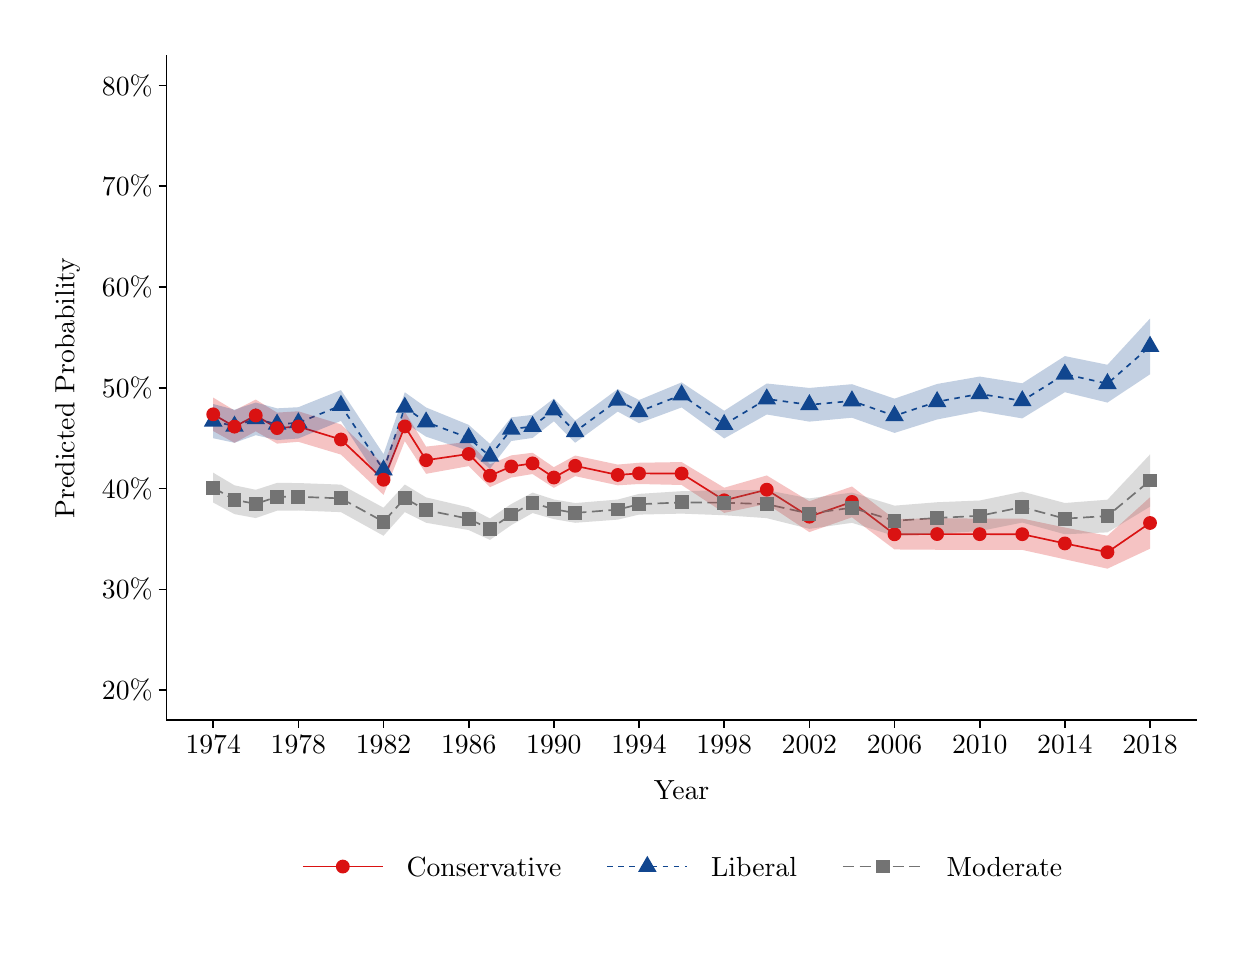
\begin{tikzpicture}[x=1pt,y=1pt]
\definecolor{fillColor}{RGB}{255,255,255}
\path[use as bounding box,fill=fillColor,fill opacity=0.00] (0,0) rectangle (432.48,324.36);
\begin{scope}
\path[clip] (  0.00,  0.00) rectangle (432.48,324.36);
\definecolor{fillColor}{RGB}{255,255,255}

\path[fill=fillColor] ( -0.00,  0.00) rectangle (432.48,324.36);
\end{scope}
\begin{scope}
\path[clip] ( 50.11, 74.07) rectangle (422.48,314.36);
\definecolor{fillColor}{RGB}{255,255,255}

\path[fill=fillColor] ( 50.11, 74.07) rectangle (422.48,314.36);
\definecolor{drawColor}{RGB}{218,18,18}

\path[draw=drawColor,line width= 0.6pt,line join=round] ( 67.04,184.64) --
	( 74.73,180.19) --
	( 82.42,184.23) --
	( 90.12,179.66) --
	( 97.81,180.23) --
	(113.20,175.55) --
	(128.59,161.00) --
	(136.28,180.27) --
	(143.97,168.06) --
	(159.36,170.32) --
	(167.05,162.46) --
	(174.75,165.80) --
	(182.44,166.91) --
	(190.13,161.80) --
	(197.83,166.03) --
	(213.22,162.74) --
	(220.91,163.30) --
	(236.30,163.25) --
	(251.68,153.57) --
	(267.07,157.41) --
	(282.46,147.65) --
	(297.85,152.99) --
	(313.23,141.29) --
	(328.62,141.37) --
	(344.01,141.34) --
	(359.39,141.32) --
	(374.78,137.99) --
	(390.17,134.82) --
	(405.56,145.38);
\definecolor{drawColor}{RGB}{17,70,143}

\path[draw=drawColor,line width= 0.6pt,dash pattern=on 2pt off 2pt ,line join=round] ( 67.04,182.18) --
	( 74.73,180.33) --
	( 82.42,183.00) --
	( 90.12,181.07) --
	( 97.81,181.56) --
	(113.20,187.83) --
	(128.59,164.48) --
	(136.28,187.15) --
	(143.97,181.84) --
	(159.36,176.13) --
	(167.05,169.45) --
	(174.75,179.27) --
	(182.44,180.27) --
	(190.13,186.23) --
	(197.83,178.37) --
	(213.22,189.70) --
	(220.91,185.62) --
	(236.30,191.66) --
	(251.68,180.92) --
	(267.07,190.18) --
	(282.46,188.09) --
	(297.85,189.47) --
	(313.23,184.11) --
	(328.62,189.20) --
	(344.01,192.03) --
	(359.39,189.51) --
	(374.78,199.15) --
	(390.17,195.72) --
	(405.56,209.18);
\definecolor{drawColor}{gray}{0.45}

\path[draw=drawColor,line width= 0.6pt,dash pattern=on 4pt off 2pt ,line join=round] ( 67.04,158.16) --
	( 74.73,153.78) --
	( 82.42,152.26) --
	( 90.12,154.84) --
	( 97.81,154.85) --
	(113.20,154.27) --
	(128.59,145.83) --
	(136.28,154.31) --
	(143.97,150.03) --
	(159.36,146.92) --
	(167.05,143.13) --
	(174.75,148.42) --
	(182.44,152.66) --
	(190.13,150.32) --
	(197.83,149.01) --
	(213.22,150.21) --
	(220.91,152.15) --
	(236.30,152.82) --
	(251.68,152.70) --
	(267.07,152.18) --
	(282.46,148.76) --
	(297.85,150.90) --
	(313.23,146.17) --
	(328.62,147.19) --
	(344.01,147.97) --
	(359.39,151.11) --
	(374.78,146.95) --
	(390.17,147.89) --
	(405.56,160.70);
\definecolor{fillColor}{RGB}{218,18,18}

\path[fill=fillColor,fill opacity=0.25] ( 67.04,190.68) --
	( 74.73,186.05) --
	( 82.42,189.97) --
	( 90.12,185.26) --
	( 97.81,185.74) --
	(113.20,181.00) --
	(128.59,166.49) --
	(136.28,185.59) --
	(143.97,172.97) --
	(159.36,174.70) --
	(167.05,166.60) --
	(174.75,169.80) --
	(182.44,170.75) --
	(190.13,165.54) --
	(197.83,169.75) --
	(213.22,166.48) --
	(220.91,167.14) --
	(236.30,167.39) --
	(251.68,158.12) --
	(267.07,162.55) --
	(282.46,153.22) --
	(297.85,158.56) --
	(313.23,146.77) --
	(328.62,147.04) --
	(344.01,146.98) --
	(359.39,146.98) --
	(374.78,143.74) --
	(390.17,140.77) --
	(405.56,154.67) --
	(405.56,136.09) --
	(390.17,128.87) --
	(374.78,132.25) --
	(359.39,135.66) --
	(344.01,135.69) --
	(328.62,135.70) --
	(313.23,135.81) --
	(297.85,147.42) --
	(282.46,142.09) --
	(267.07,152.27) --
	(251.68,149.02) --
	(236.30,159.11) --
	(220.91,159.46) --
	(213.22,158.99) --
	(197.83,162.31) --
	(190.13,158.07) --
	(182.44,163.07) --
	(174.75,161.80) --
	(167.05,158.32) --
	(159.36,165.93) --
	(143.97,163.15) --
	(136.28,174.96) --
	(128.59,155.51) --
	(113.20,170.10) --
	( 97.81,174.71) --
	( 90.12,174.06) --
	( 82.42,178.50) --
	( 74.73,174.34) --
	( 67.04,178.59) --
	cycle;

\path[] ( 67.04,190.68) --
	( 74.73,186.05) --
	( 82.42,189.97) --
	( 90.12,185.26) --
	( 97.81,185.74) --
	(113.20,181.00) --
	(128.59,166.49) --
	(136.28,185.59) --
	(143.97,172.97) --
	(159.36,174.70) --
	(167.05,166.60) --
	(174.75,169.80) --
	(182.44,170.75) --
	(190.13,165.54) --
	(197.83,169.75) --
	(213.22,166.48) --
	(220.91,167.14) --
	(236.30,167.39) --
	(251.68,158.12) --
	(267.07,162.55) --
	(282.46,153.22) --
	(297.85,158.56) --
	(313.23,146.77) --
	(328.62,147.04) --
	(344.01,146.98) --
	(359.39,146.98) --
	(374.78,143.74) --
	(390.17,140.77) --
	(405.56,154.67);

\path[] (405.56,136.09) --
	(390.17,128.87) --
	(374.78,132.25) --
	(359.39,135.66) --
	(344.01,135.69) --
	(328.62,135.70) --
	(313.23,135.81) --
	(297.85,147.42) --
	(282.46,142.09) --
	(267.07,152.27) --
	(251.68,149.02) --
	(236.30,159.11) --
	(220.91,159.46) --
	(213.22,158.99) --
	(197.83,162.31) --
	(190.13,158.07) --
	(182.44,163.07) --
	(174.75,161.80) --
	(167.05,158.32) --
	(159.36,165.93) --
	(143.97,163.15) --
	(136.28,174.96) --
	(128.59,155.51) --
	(113.20,170.10) --
	( 97.81,174.71) --
	( 90.12,174.06) --
	( 82.42,178.50) --
	( 74.73,174.34) --
	( 67.04,178.59);
\definecolor{fillColor}{RGB}{17,70,143}

\path[fill=fillColor,fill opacity=0.25] ( 67.04,188.36) --
	( 74.73,186.31) --
	( 82.42,188.91) --
	( 90.12,186.80) --
	( 97.81,187.21) --
	(113.20,193.39) --
	(128.59,170.25) --
	(136.28,192.61) --
	(143.97,187.11) --
	(159.36,180.83) --
	(167.05,173.95) --
	(174.75,183.54) --
	(182.44,184.44) --
	(190.13,190.35) --
	(197.83,182.37) --
	(213.22,193.78) --
	(220.91,189.80) --
	(236.30,196.18) --
	(251.68,185.92) --
	(267.07,195.77) --
	(282.46,194.17) --
	(297.85,195.52) --
	(313.23,190.31) --
	(328.62,195.61) --
	(344.01,198.29) --
	(359.39,195.84) --
	(374.78,205.68) --
	(390.17,202.55) --
	(405.56,219.25) --
	(405.56,199.11) --
	(390.17,188.89) --
	(374.78,192.63) --
	(359.39,183.17) --
	(344.01,185.77) --
	(328.62,182.78) --
	(313.23,177.92) --
	(297.85,183.41) --
	(282.46,182.01) --
	(267.07,184.58) --
	(251.68,175.93) --
	(236.30,187.13) --
	(220.91,181.43) --
	(213.22,185.63) --
	(197.83,174.37) --
	(190.13,182.11) --
	(182.44,176.11) --
	(174.75,175.00) --
	(167.05,164.96) --
	(159.36,171.44) --
	(143.97,176.57) --
	(136.28,181.69) --
	(128.59,158.71) --
	(113.20,182.27) --
	( 97.81,175.91) --
	( 90.12,175.34) --
	( 82.42,177.10) --
	( 74.73,174.36) --
	( 67.04,176.00) --
	cycle;

\path[] ( 67.04,188.36) --
	( 74.73,186.31) --
	( 82.42,188.91) --
	( 90.12,186.80) --
	( 97.81,187.21) --
	(113.20,193.39) --
	(128.59,170.25) --
	(136.28,192.61) --
	(143.97,187.11) --
	(159.36,180.83) --
	(167.05,173.95) --
	(174.75,183.54) --
	(182.44,184.44) --
	(190.13,190.35) --
	(197.83,182.37) --
	(213.22,193.78) --
	(220.91,189.80) --
	(236.30,196.18) --
	(251.68,185.92) --
	(267.07,195.77) --
	(282.46,194.17) --
	(297.85,195.52) --
	(313.23,190.31) --
	(328.62,195.61) --
	(344.01,198.29) --
	(359.39,195.84) --
	(374.78,205.68) --
	(390.17,202.55) --
	(405.56,219.25);

\path[] (405.56,199.11) --
	(390.17,188.89) --
	(374.78,192.63) --
	(359.39,183.17) --
	(344.01,185.77) --
	(328.62,182.78) --
	(313.23,177.92) --
	(297.85,183.41) --
	(282.46,182.01) --
	(267.07,184.58) --
	(251.68,175.93) --
	(236.30,187.13) --
	(220.91,181.43) --
	(213.22,185.63) --
	(197.83,174.37) --
	(190.13,182.11) --
	(182.44,176.11) --
	(174.75,175.00) --
	(167.05,164.96) --
	(159.36,171.44) --
	(143.97,176.57) --
	(136.28,181.69) --
	(128.59,158.71) --
	(113.20,182.27) --
	( 97.81,175.91) --
	( 90.12,175.34) --
	( 82.42,177.10) --
	( 74.73,174.36) --
	( 67.04,176.00);
\definecolor{fillColor}{RGB}{115,115,115}

\path[fill=fillColor,fill opacity=0.25] ( 67.04,163.54) --
	( 74.73,158.98) --
	( 82.42,157.37) --
	( 90.12,159.86) --
	( 97.81,159.81) --
	(113.20,159.24) --
	(128.59,150.90) --
	(136.28,159.28) --
	(143.97,154.62) --
	(159.36,151.03) --
	(167.05,147.00) --
	(174.75,152.23) --
	(182.44,156.36) --
	(190.13,153.87) --
	(197.83,152.58) --
	(213.22,153.84) --
	(220.91,155.89) --
	(236.30,156.87) --
	(251.68,157.23) --
	(267.07,157.23) --
	(282.46,154.26) --
	(297.85,156.37) --
	(313.23,151.64) --
	(328.62,152.87) --
	(344.01,153.50) --
	(359.39,156.69) --
	(374.78,152.60) --
	(390.17,153.79) --
	(405.56,170.15) --
	(405.56,151.26) --
	(390.17,141.99) --
	(374.78,141.30) --
	(359.39,145.53) --
	(344.01,142.44) --
	(328.62,141.51) --
	(313.23,140.69) --
	(297.85,145.43) --
	(282.46,143.26) --
	(267.07,147.13) --
	(251.68,148.18) --
	(236.30,148.76) --
	(220.91,148.41) --
	(213.22,146.59) --
	(197.83,145.45) --
	(190.13,146.77) --
	(182.44,148.97) --
	(174.75,144.60) --
	(167.05,139.27) --
	(159.36,142.82) --
	(143.97,145.45) --
	(136.28,149.33) --
	(128.59,140.76) --
	(113.20,149.30) --
	( 97.81,149.89) --
	( 90.12,149.82) --
	( 82.42,147.15) --
	( 74.73,148.58) --
	( 67.04,152.77) --
	cycle;

\path[] ( 67.04,163.54) --
	( 74.73,158.98) --
	( 82.42,157.37) --
	( 90.12,159.86) --
	( 97.81,159.81) --
	(113.20,159.24) --
	(128.59,150.90) --
	(136.28,159.28) --
	(143.97,154.62) --
	(159.36,151.03) --
	(167.05,147.00) --
	(174.75,152.23) --
	(182.44,156.36) --
	(190.13,153.87) --
	(197.83,152.58) --
	(213.22,153.84) --
	(220.91,155.89) --
	(236.30,156.87) --
	(251.68,157.23) --
	(267.07,157.23) --
	(282.46,154.26) --
	(297.85,156.37) --
	(313.23,151.64) --
	(328.62,152.87) --
	(344.01,153.50) --
	(359.39,156.69) --
	(374.78,152.60) --
	(390.17,153.79) --
	(405.56,170.15);

\path[] (405.56,151.26) --
	(390.17,141.99) --
	(374.78,141.30) --
	(359.39,145.53) --
	(344.01,142.44) --
	(328.62,141.51) --
	(313.23,140.69) --
	(297.85,145.43) --
	(282.46,143.26) --
	(267.07,147.13) --
	(251.68,148.18) --
	(236.30,148.76) --
	(220.91,148.41) --
	(213.22,146.59) --
	(197.83,145.45) --
	(190.13,146.77) --
	(182.44,148.97) --
	(174.75,144.60) --
	(167.05,139.27) --
	(159.36,142.82) --
	(143.97,145.45) --
	(136.28,149.33) --
	(128.59,140.76) --
	(113.20,149.30) --
	( 97.81,149.89) --
	( 90.12,149.82) --
	( 82.42,147.15) --
	( 74.73,148.58) --
	( 67.04,152.77);
\definecolor{fillColor}{RGB}{17,70,143}

\path[fill=fillColor] ( 67.04,186.07) --
	( 70.40,180.24) --
	( 63.67,180.24) --
	cycle;

\path[fill=fillColor] ( 74.73,184.22) --
	( 78.09,178.39) --
	( 71.37,178.39) --
	cycle;

\path[fill=fillColor] ( 82.42,186.89) --
	( 85.79,181.06) --
	( 79.06,181.06) --
	cycle;

\path[fill=fillColor] ( 90.12,184.95) --
	( 93.48,179.13) --
	( 86.75,179.13) --
	cycle;

\path[fill=fillColor] ( 97.81,185.44) --
	(101.17,179.62) --
	( 94.45,179.62) --
	cycle;

\path[fill=fillColor] (113.20,191.72) --
	(116.56,185.89) --
	(109.83,185.89) --
	cycle;

\path[fill=fillColor] (128.59,168.37) --
	(131.95,162.54) --
	(125.22,162.54) --
	cycle;

\path[fill=fillColor] (136.28,191.04) --
	(139.64,185.21) --
	(132.91,185.21) --
	cycle;

\path[fill=fillColor] (143.97,185.72) --
	(147.34,179.90) --
	(140.61,179.90) --
	cycle;

\path[fill=fillColor] (159.36,180.02) --
	(162.72,174.19) --
	(156.00,174.19) --
	cycle;

\path[fill=fillColor] (167.05,173.34) --
	(170.42,167.51) --
	(163.69,167.51) --
	cycle;

\path[fill=fillColor] (174.75,183.16) --
	(178.11,177.33) --
	(171.38,177.33) --
	cycle;

\path[fill=fillColor] (182.44,184.16) --
	(185.80,178.33) --
	(179.08,178.33) --
	cycle;

\path[fill=fillColor] (190.13,190.11) --
	(193.50,184.29) --
	(186.77,184.29) --
	cycle;

\path[fill=fillColor] (197.83,182.25) --
	(201.19,176.43) --
	(194.46,176.43) --
	cycle;

\path[fill=fillColor] (213.22,193.59) --
	(216.58,187.76) --
	(209.85,187.76) --
	cycle;

\path[fill=fillColor] (220.91,189.50) --
	(224.27,183.67) --
	(217.54,183.67) --
	cycle;

\path[fill=fillColor] (236.30,195.54) --
	(239.66,189.71) --
	(232.93,189.71) --
	cycle;

\path[fill=fillColor] (251.68,184.81) --
	(255.05,178.98) --
	(248.32,178.98) --
	cycle;

\path[fill=fillColor] (267.07,194.06) --
	(270.43,188.23) --
	(263.71,188.23) --
	cycle;

\path[fill=fillColor] (282.46,191.98) --
	(285.82,186.15) --
	(279.09,186.15) --
	cycle;

\path[fill=fillColor] (297.85,193.35) --
	(301.21,187.52) --
	(294.48,187.52) --
	cycle;

\path[fill=fillColor] (313.23,188.00) --
	(316.60,182.17) --
	(309.87,182.17) --
	cycle;

\path[fill=fillColor] (328.62,193.08) --
	(331.98,187.25) --
	(325.26,187.25) --
	cycle;

\path[fill=fillColor] (344.01,195.91) --
	(347.37,190.09) --
	(340.64,190.09) --
	cycle;

\path[fill=fillColor] (359.39,193.39) --
	(362.76,187.57) --
	(356.03,187.57) --
	cycle;

\path[fill=fillColor] (374.78,203.04) --
	(378.15,197.21) --
	(371.42,197.21) --
	cycle;

\path[fill=fillColor] (390.17,199.61) --
	(393.53,193.78) --
	(386.80,193.78) --
	cycle;

\path[fill=fillColor] (405.56,213.06) --
	(408.92,207.24) --
	(402.19,207.24) --
	cycle;
\definecolor{fillColor}{RGB}{218,18,18}

\path[fill=fillColor] ( 67.04,184.64) circle (  2.50);

\path[fill=fillColor] ( 74.73,180.19) circle (  2.50);

\path[fill=fillColor] ( 82.42,184.23) circle (  2.50);

\path[fill=fillColor] ( 90.12,179.66) circle (  2.50);

\path[fill=fillColor] ( 97.81,180.23) circle (  2.50);

\path[fill=fillColor] (113.20,175.55) circle (  2.50);

\path[fill=fillColor] (128.59,161.00) circle (  2.50);

\path[fill=fillColor] (136.28,180.27) circle (  2.50);

\path[fill=fillColor] (143.97,168.06) circle (  2.50);

\path[fill=fillColor] (159.36,170.32) circle (  2.50);

\path[fill=fillColor] (167.05,162.46) circle (  2.50);

\path[fill=fillColor] (174.75,165.80) circle (  2.50);

\path[fill=fillColor] (182.44,166.91) circle (  2.50);

\path[fill=fillColor] (190.13,161.80) circle (  2.50);

\path[fill=fillColor] (197.83,166.03) circle (  2.50);

\path[fill=fillColor] (213.22,162.74) circle (  2.50);

\path[fill=fillColor] (220.91,163.30) circle (  2.50);

\path[fill=fillColor] (236.30,163.25) circle (  2.50);

\path[fill=fillColor] (251.68,153.57) circle (  2.50);

\path[fill=fillColor] (267.07,157.41) circle (  2.50);

\path[fill=fillColor] (282.46,147.65) circle (  2.50);

\path[fill=fillColor] (297.85,152.99) circle (  2.50);

\path[fill=fillColor] (313.23,141.29) circle (  2.50);

\path[fill=fillColor] (328.62,141.37) circle (  2.50);

\path[fill=fillColor] (344.01,141.34) circle (  2.50);

\path[fill=fillColor] (359.39,141.32) circle (  2.50);

\path[fill=fillColor] (374.78,137.99) circle (  2.50);

\path[fill=fillColor] (390.17,134.82) circle (  2.50);

\path[fill=fillColor] (405.56,145.38) circle (  2.50);
\definecolor{fillColor}{gray}{0.45}

\path[fill=fillColor] ( 64.54,155.66) --
	( 69.53,155.66) --
	( 69.53,160.66) --
	( 64.54,160.66) --
	cycle;

\path[fill=fillColor] ( 72.23,151.28) --
	( 77.23,151.28) --
	( 77.23,156.27) --
	( 72.23,156.27) --
	cycle;

\path[fill=fillColor] ( 79.93,149.77) --
	( 84.92,149.77) --
	( 84.92,154.76) --
	( 79.93,154.76) --
	cycle;

\path[fill=fillColor] ( 87.62,152.34) --
	( 92.61,152.34) --
	( 92.61,157.33) --
	( 87.62,157.33) --
	cycle;

\path[fill=fillColor] ( 95.31,152.35) --
	(100.31,152.35) --
	(100.31,157.35) --
	( 95.31,157.35) --
	cycle;

\path[fill=fillColor] (110.70,151.77) --
	(115.70,151.77) --
	(115.70,156.76) --
	(110.70,156.76) --
	cycle;

\path[fill=fillColor] (126.09,143.33) --
	(131.08,143.33) --
	(131.08,148.33) --
	(126.09,148.33) --
	cycle;

\path[fill=fillColor] (133.78,151.81) --
	(138.78,151.81) --
	(138.78,156.81) --
	(133.78,156.81) --
	cycle;

\path[fill=fillColor] (141.47,147.53) --
	(146.47,147.53) --
	(146.47,152.53) --
	(141.47,152.53) --
	cycle;

\path[fill=fillColor] (156.86,144.43) --
	(161.86,144.43) --
	(161.86,149.42) --
	(156.86,149.42) --
	cycle;

\path[fill=fillColor] (164.56,140.63) --
	(169.55,140.63) --
	(169.55,145.63) --
	(164.56,145.63) --
	cycle;

\path[fill=fillColor] (172.25,145.92) --
	(177.24,145.92) --
	(177.24,150.91) --
	(172.25,150.91) --
	cycle;

\path[fill=fillColor] (179.94,150.16) --
	(184.94,150.16) --
	(184.94,155.16) --
	(179.94,155.16) --
	cycle;

\path[fill=fillColor] (187.64,147.82) --
	(192.63,147.82) --
	(192.63,152.82) --
	(187.64,152.82) --
	cycle;

\path[fill=fillColor] (195.33,146.52) --
	(200.33,146.52) --
	(200.33,151.51) --
	(195.33,151.51) --
	cycle;

\path[fill=fillColor] (210.72,147.72) --
	(215.71,147.72) --
	(215.71,152.71) --
	(210.72,152.71) --
	cycle;

\path[fill=fillColor] (218.41,149.65) --
	(223.41,149.65) --
	(223.41,154.65) --
	(218.41,154.65) --
	cycle;

\path[fill=fillColor] (233.80,150.32) --
	(238.79,150.32) --
	(238.79,155.32) --
	(233.80,155.32) --
	cycle;

\path[fill=fillColor] (249.19,150.21) --
	(254.18,150.21) --
	(254.18,155.20) --
	(249.19,155.20) --
	cycle;

\path[fill=fillColor] (264.57,149.68) --
	(269.57,149.68) --
	(269.57,154.68) --
	(264.57,154.68) --
	cycle;

\path[fill=fillColor] (279.96,146.27) --
	(284.96,146.27) --
	(284.96,151.26) --
	(279.96,151.26) --
	cycle;

\path[fill=fillColor] (295.35,148.40) --
	(300.34,148.40) --
	(300.34,153.40) --
	(295.35,153.40) --
	cycle;

\path[fill=fillColor] (310.73,143.67) --
	(315.73,143.67) --
	(315.73,148.66) --
	(310.73,148.66) --
	cycle;

\path[fill=fillColor] (326.12,144.69) --
	(331.12,144.69) --
	(331.12,149.69) --
	(326.12,149.69) --
	cycle;

\path[fill=fillColor] (341.51,145.48) --
	(346.50,145.48) --
	(346.50,150.47) --
	(341.51,150.47) --
	cycle;

\path[fill=fillColor] (356.90,148.61) --
	(361.89,148.61) --
	(361.89,153.61) --
	(356.90,153.61) --
	cycle;

\path[fill=fillColor] (372.28,144.45) --
	(377.28,144.45) --
	(377.28,149.45) --
	(372.28,149.45) --
	cycle;

\path[fill=fillColor] (387.67,145.39) --
	(392.67,145.39) --
	(392.67,150.39) --
	(387.67,150.39) --
	cycle;

\path[fill=fillColor] (403.06,158.20) --
	(408.05,158.20) --
	(408.05,163.20) --
	(403.06,163.20) --
	cycle;
\end{scope}
\begin{scope}
\path[clip] (  0.00,  0.00) rectangle (432.48,324.36);
\definecolor{drawColor}{RGB}{0,0,0}

\path[draw=drawColor,line width= 0.6pt,line join=round] ( 50.11, 74.07) --
	( 50.11,314.36);
\end{scope}
\begin{scope}
\path[clip] (  0.00,  0.00) rectangle (432.48,324.36);
\definecolor{drawColor}{RGB}{0,0,0}

\node[text=drawColor,anchor=base east,inner sep=0pt, outer sep=0pt, scale=  1.00] at ( 45.16, 81.55) {20{\%}};

\node[text=drawColor,anchor=base east,inner sep=0pt, outer sep=0pt, scale=  1.00] at ( 45.16,117.95) {30{\%}};

\node[text=drawColor,anchor=base east,inner sep=0pt, outer sep=0pt, scale=  1.00] at ( 45.16,154.36) {40{\%}};

\node[text=drawColor,anchor=base east,inner sep=0pt, outer sep=0pt, scale=  1.00] at ( 45.16,190.77) {50{\%}};

\node[text=drawColor,anchor=base east,inner sep=0pt, outer sep=0pt, scale=  1.00] at ( 45.16,227.18) {60{\%}};

\node[text=drawColor,anchor=base east,inner sep=0pt, outer sep=0pt, scale=  1.00] at ( 45.16,263.59) {70{\%}};

\node[text=drawColor,anchor=base east,inner sep=0pt, outer sep=0pt, scale=  1.00] at ( 45.16,300.00) {80{\%}};
\end{scope}
\begin{scope}
\path[clip] (  0.00,  0.00) rectangle (432.48,324.36);
\definecolor{drawColor}{RGB}{0,0,0}

\path[draw=drawColor,line width= 0.6pt,line join=round] ( 47.36, 84.99) --
	( 50.11, 84.99);

\path[draw=drawColor,line width= 0.6pt,line join=round] ( 47.36,121.40) --
	( 50.11,121.40);

\path[draw=drawColor,line width= 0.6pt,line join=round] ( 47.36,157.81) --
	( 50.11,157.81);

\path[draw=drawColor,line width= 0.6pt,line join=round] ( 47.36,194.21) --
	( 50.11,194.21);

\path[draw=drawColor,line width= 0.6pt,line join=round] ( 47.36,230.62) --
	( 50.11,230.62);

\path[draw=drawColor,line width= 0.6pt,line join=round] ( 47.36,267.03) --
	( 50.11,267.03);

\path[draw=drawColor,line width= 0.6pt,line join=round] ( 47.36,303.44) --
	( 50.11,303.44);
\end{scope}
\begin{scope}
\path[clip] (  0.00,  0.00) rectangle (432.48,324.36);
\definecolor{drawColor}{RGB}{0,0,0}

\path[draw=drawColor,line width= 0.6pt,line join=round] ( 50.11, 74.07) --
	(422.48, 74.07);
\end{scope}
\begin{scope}
\path[clip] (  0.00,  0.00) rectangle (432.48,324.36);
\definecolor{drawColor}{RGB}{0,0,0}

\path[draw=drawColor,line width= 0.6pt,line join=round] ( 67.04, 71.32) --
	( 67.04, 74.07);

\path[draw=drawColor,line width= 0.6pt,line join=round] ( 97.81, 71.32) --
	( 97.81, 74.07);

\path[draw=drawColor,line width= 0.6pt,line join=round] (128.59, 71.32) --
	(128.59, 74.07);

\path[draw=drawColor,line width= 0.6pt,line join=round] (159.36, 71.32) --
	(159.36, 74.07);

\path[draw=drawColor,line width= 0.6pt,line join=round] (190.13, 71.32) --
	(190.13, 74.07);

\path[draw=drawColor,line width= 0.6pt,line join=round] (220.91, 71.32) --
	(220.91, 74.07);

\path[draw=drawColor,line width= 0.6pt,line join=round] (251.68, 71.32) --
	(251.68, 74.07);

\path[draw=drawColor,line width= 0.6pt,line join=round] (282.46, 71.32) --
	(282.46, 74.07);

\path[draw=drawColor,line width= 0.6pt,line join=round] (313.23, 71.32) --
	(313.23, 74.07);

\path[draw=drawColor,line width= 0.6pt,line join=round] (344.01, 71.32) --
	(344.01, 74.07);

\path[draw=drawColor,line width= 0.6pt,line join=round] (374.78, 71.32) --
	(374.78, 74.07);

\path[draw=drawColor,line width= 0.6pt,line join=round] (405.56, 71.32) --
	(405.56, 74.07);
\end{scope}
\begin{scope}
\path[clip] (  0.00,  0.00) rectangle (432.48,324.36);
\definecolor{drawColor}{RGB}{0,0,0}

\node[text=drawColor,anchor=base,inner sep=0pt, outer sep=0pt, scale=  1.00] at ( 67.04, 62.23) {1974};

\node[text=drawColor,anchor=base,inner sep=0pt, outer sep=0pt, scale=  1.00] at ( 97.81, 62.23) {1978};

\node[text=drawColor,anchor=base,inner sep=0pt, outer sep=0pt, scale=  1.00] at (128.59, 62.23) {1982};

\node[text=drawColor,anchor=base,inner sep=0pt, outer sep=0pt, scale=  1.00] at (159.36, 62.23) {1986};

\node[text=drawColor,anchor=base,inner sep=0pt, outer sep=0pt, scale=  1.00] at (190.13, 62.23) {1990};

\node[text=drawColor,anchor=base,inner sep=0pt, outer sep=0pt, scale=  1.00] at (220.91, 62.23) {1994};

\node[text=drawColor,anchor=base,inner sep=0pt, outer sep=0pt, scale=  1.00] at (251.68, 62.23) {1998};

\node[text=drawColor,anchor=base,inner sep=0pt, outer sep=0pt, scale=  1.00] at (282.46, 62.23) {2002};

\node[text=drawColor,anchor=base,inner sep=0pt, outer sep=0pt, scale=  1.00] at (313.23, 62.23) {2006};

\node[text=drawColor,anchor=base,inner sep=0pt, outer sep=0pt, scale=  1.00] at (344.01, 62.23) {2010};

\node[text=drawColor,anchor=base,inner sep=0pt, outer sep=0pt, scale=  1.00] at (374.78, 62.23) {2014};

\node[text=drawColor,anchor=base,inner sep=0pt, outer sep=0pt, scale=  1.00] at (405.56, 62.23) {2018};
\end{scope}
\begin{scope}
\path[clip] (  0.00,  0.00) rectangle (432.48,324.36);
\definecolor{drawColor}{RGB}{0,0,0}

\node[text=drawColor,anchor=base,inner sep=0pt, outer sep=0pt, scale=  1.00] at (236.30, 45.40) {Year};
\end{scope}
\begin{scope}
\path[clip] (  0.00,  0.00) rectangle (432.48,324.36);
\definecolor{drawColor}{RGB}{0,0,0}

\node[text=drawColor,rotate= 90.00,anchor=base,inner sep=0pt, outer sep=0pt, scale=  1.00] at ( 16.89,194.21) {Predicted Probability};
\end{scope}
\begin{scope}
\path[clip] (  0.00,  0.00) rectangle (432.48,324.36);

\path[] ( 86.80, 10.00) rectangle (385.79, 32.45);
\end{scope}
\begin{scope}
\path[clip] (  0.00,  0.00) rectangle (432.48,324.36);

\path[] ( 95.80, 14.00) rectangle (131.94, 28.45);
\end{scope}
\begin{scope}
\path[clip] (  0.00,  0.00) rectangle (432.48,324.36);
\definecolor{drawColor}{RGB}{218,18,18}

\path[draw=drawColor,line width= 0.6pt,line join=round] ( 99.42, 21.23) -- (128.33, 21.23);
\end{scope}
\begin{scope}
\path[clip] (  0.00,  0.00) rectangle (432.48,324.36);
\definecolor{fillColor}{RGB}{218,18,18}

\path[fill=fillColor] (113.87, 21.23) circle (  2.50);
\end{scope}
\begin{scope}
\path[clip] (  0.00,  0.00) rectangle (432.48,324.36);

\path[] (205.84, 14.00) rectangle (241.98, 28.45);
\end{scope}
\begin{scope}
\path[clip] (  0.00,  0.00) rectangle (432.48,324.36);
\definecolor{drawColor}{RGB}{17,70,143}

\path[draw=drawColor,line width= 0.6pt,dash pattern=on 2pt off 2pt ,line join=round] (209.46, 21.23) -- (238.36, 21.23);
\end{scope}
\begin{scope}
\path[clip] (  0.00,  0.00) rectangle (432.48,324.36);
\definecolor{fillColor}{RGB}{17,70,143}

\path[fill=fillColor] (223.91, 25.11) --
	(227.27, 19.28) --
	(220.55, 19.28) --
	cycle;
\end{scope}
\begin{scope}
\path[clip] (  0.00,  0.00) rectangle (432.48,324.36);

\path[] (290.97, 14.00) rectangle (327.10, 28.45);
\end{scope}
\begin{scope}
\path[clip] (  0.00,  0.00) rectangle (432.48,324.36);
\definecolor{drawColor}{gray}{0.45}

\path[draw=drawColor,line width= 0.6pt,dash pattern=on 4pt off 2pt ,line join=round] (294.58, 21.23) -- (323.49, 21.23);
\end{scope}
\begin{scope}
\path[clip] (  0.00,  0.00) rectangle (432.48,324.36);
\definecolor{fillColor}{gray}{0.45}

\path[fill=fillColor] (306.54, 18.73) --
	(311.53, 18.73) --
	(311.53, 23.72) --
	(306.54, 23.72) --
	cycle;
\end{scope}
\begin{scope}
\path[clip] (  0.00,  0.00) rectangle (432.48,324.36);
\definecolor{drawColor}{RGB}{0,0,0}

\node[text=drawColor,anchor=base west,inner sep=0pt, outer sep=0pt, scale=  1.00] at (136.94, 17.78) {Conservative};
\end{scope}
\begin{scope}
\path[clip] (  0.00,  0.00) rectangle (432.48,324.36);
\definecolor{drawColor}{RGB}{0,0,0}

\node[text=drawColor,anchor=base west,inner sep=0pt, outer sep=0pt, scale=  1.00] at (246.98, 17.78) {Liberal};
\end{scope}
\begin{scope}
\path[clip] (  0.00,  0.00) rectangle (432.48,324.36);
\definecolor{drawColor}{RGB}{0,0,0}

\node[text=drawColor,anchor=base west,inner sep=0pt, outer sep=0pt, scale=  1.00] at (332.10, 17.78) {Moderate};
\end{scope}
\end{tikzpicture}
